\section{Электрон-фононное взаимодействие}
В данном разделе мы рассмотрим модель электрон-фононного взаимодействия,
которая позволяет правильно описать температурные зависимости спектра. 
По существу, электрон-фононное взаимодействие аналогично электрон-фотонному.
Есть известные выражениия для распределения фононов по энергиям при заданной
температуре (распределение Бозе-Эйнштейна), которое, в конечном счёте, используется
для нахождения соответствующих характеристик спектра.

Невозмущённый гамильтониан спин-орбитального взаимодействия для нулевого и первого
возмущённого уровней с заданным спином даётся формулой \ref{H_0}. 
Здесь $\hbar \Delta$ -- величина соответствующего тонкого расщепления,
$\sigma_z$ -- матрица Паули. Отметим, что электрон-фононное взаимодействие не 
изменяет спинового состояния электрона, поэтому можно рассматривать тонкое расщепление
с одним заданным спиновым состоянием, но с разными проекциями момента импульса.

\begin{equation}
    \label{H_0}
    H_0 = \pm \frac{1}{2} \hbar \Delta \sigma_z.
\end{equation}

Гамильтониан фононного газа описывается формулой \ref{H_P}. Здесь суммирование
проводится по двум поляризациям $p$ и по всем волновым векторам $k$; $\hbar \omega_k$ --
энергия соответствующего фонона с волновым вектором $k$, $a^{\dagger}_{p, k}$ и
$a_{p, k}$ -- операторы рождения и уничтожения. 

\begin{equation}
    \label{H_P}
    \hat{H}_P = \sum_{p, k} \hbar \omega_k a^{\dagger}_{p, k} a_{p, k}.
\end{equation}

Формула \ref{V_{e-p}} задаёт возмущение, вызванное электрон-фононным взаимодействием.
Здесь $\sigma_{-} и \sigma_{+}$ -- соответствующие операторы повышения и понижения
орибтального состояния электрона. Ясно, что определённое изменение орбитального момента
электрона сопровождается поглощением фонона с определённой поляризацией. Коэффициент
$\chi_k$ задаёт частоту электрон-фононного взаимодействия. Известно, что 
$\overline{|\chi_k|^2} \approx \chi \omega$, где $\chi$ -- константа. Усреднение берётся
по всем модам $k$ с частотой $\omega$.

\begin{equation}
    \label{V_{e-p}}
    \hat{V}_{e-p} = \sum_{k} \hbar \chi_k \left[\sigma_{+}\left(a_{-, k}
    + a^{\dagger}_{-, k} \right) + \sigma_{-} \left(a_{+, k} + a^{\dagger}_{+, k}
     \right)   \right].
\end{equation}


\subsection{Первый порядок возмущения}
Рассмотрим \ref{V_{e-p}} как возмущение, зависящее от времени. Тогда в первом порядке
малости имеем выражения для скоростей переходов \ref{Gamma+} и \ref{Gamma-}. 
Эти величины соответствуют обратной величине времени релаксации, соответственно,
именно они задают характерную ширину уровня. Здесь $n_{-, k}$-- количество 
фононов с соответствующей поляризацией и волновым вектором, $\delta$ -- дельта-функция
Дирака. Заметим, что данные переходы соответвуют однофононному поглощению (случай (а)
на рис. \ref{J-T effect}).

\begin{equation}
    \label{Gamma+}
    \gamma_+ = 2\pi \sum_{k}n_{-, k}|\chi_k^2|\delta (\Delta - \omega_k),
\end{equation}

\begin{equation}
    \label{Gamma-}
    \gamma_- = 2\pi \sum_{k}(n_{+, k}+1)|\chi_k^2|\delta (\Delta - \omega_k).
\end{equation}

Учитывая, что плотность состояний $\rho(\omega) = \rho \omega^2$, где $\rho$ - константа,
получаем выражения \ref{Gamma+2}, \ref{Gamma-2}. 

\begin{equation}
    \label{Gamma+2}
    \gamma_+ = 2\pi \chi \rho \Delta^3 n(\Delta, T),
\end{equation}

\begin{equation}
    \label{Gamma-2}
    \gamma_- = 2\pi \chi \rho \Delta^3 \left( n(\Delta, T)+1 \right).
\end{equation}

Распределение Бозе-Эйнштейна даётся формулой \ref{Bose-Einstain distribution}.
При больших температурах, таких, чтобы экспоненту можно было разложить в ряд Тейлора 
$T > 2.4 \text{ К}$, скорости соответствующих переходов приближённо задаются 
формулой \ref{Gamma}.

\begin{equation}
    \label{Bose-Einstain distribution}
    n(\Delta, T) = \frac{1}{\exp(\frac{\hbar \Delta}{k_{B}T})-1}.
\end{equation}

\begin{equation}
    \label{Gamma}
    \gamma_{+} \approx \gamma_{-} \approx 2\pi \chi \rho \Delta^2 \frac{k_{B}T}{\hbar}.
\end{equation}


Видно, что в первом порядке возмущения зависимость ширины линии перехода от температуры
квадратична. Однако такое рассмотрение правильно описывает экспериментальные данные
только до температур $T \sim 20 \text{ К}$. При температурах выше указанной доминирующим
становится двухфононный процесс.

\subsection{Второй порядок возмущения}
Из вида возмущения \ref{V_{e-p}} следует, что для рассматриваемых центров допускаются только
процессы рассеяния фононов (c), рис. \ref{J-T effect}, в отличие от NV-центров, где
доминирующим является Рамановский процесс (b). Однако есть в алмазе есть механическое
напряжение, то процесс (b) становится возможным и для GeV- и SiV-центров окраски. 

Во втором порядке возмущения имеем формулу \ref{Gamma_b} для скорости переходов.
Из неё также следует формула \ref{Gamma_b2}. Здесть $\Omega$ -- максимальная
частота колебаний в алмазе, или Дебаевская частота.

\begin{equation}
    \label{Gamma_b}
    \gamma_{-} = 2\pi \hbar^2 \sum_{k, q}n_{-, k}\left(n_{+, q} + 1 \right) 
    |\chi_k^2||\chi_q^2|\left|\frac{1}{\Delta - \omega_k} + \frac{1}{\Delta + \omega_k
    } \right|^2 \delta\left(\Delta - \omega_k + \omega_q \right)
\end{equation}

\begin{equation}
    \label{Gamma_b2}
    \gamma_{-} = 2 \pi \hbar^2 \int_{0}^{\Omega} n\left(\Delta + \omega, T\right)
    \left(n\left(\omega, T \right) + 1\right) \overline{\left|\gamma_k \left(
        \Delta + \omega
    \right)\right|^2}\overline{\left|\chi_q\left(\omega\right)\right|^2}\left|
    \frac{1}{\Delta - \omega} + \frac{1}{\Delta + \omega}\right|^2\rho\left(\Delta + \omega
    \right)\rho\left(\omega\right)d\omega
\end{equation}


Как известно, температура дебая для алмаза $\Theta = 2230 \text{ К}$, что позволяет
использовать приближение $\Omega \gg \omega \gg \Delta$. В таком случае формула
\ref{Gamma_b2} переходит в формулу \ref{Gamma_b_final}. Отсюда исходит, что ширина
линии зависит от температуры $\propto T^3$. 

\begin{equation}
    \label{Gamma_b_final}
    \gamma_{-} \approx \gamma_{+} \approx 2 \pi \hbar^2 \Delta^2 \chi^2 \rho^2
    \int_{0}^{\infty} n\left(\omega, T\right)\left(n\left(\omega, T\right)+1\right)
    \omega^2 d\omega = \frac{2 \pi^3}{3\hbar}\Delta^2 \chi^2 \rho^2 k_{B}^3 T^3.
\end{equation}


\subsection{Вычисление энергетических сдвигов}
Как было показано выше, здесь применима аналогия с КЭД, 
только для фононов.Электрон-фононные взаимодействия также возмущают энергии
орбитальных состояний во втором порядке теории возмущений. Сдвиги энергии во втором порядке
$\delta E_{-}$ ($\delta E_{+}$) для состояний $|e_{-}\rangle$ ($|e_{+}\rangle$)
могут быть выражены в простой форме с использованием линейного фононного $\{x, y\}$
поляризованного базиса. Сдвиг энергии из-за фононных мод с волновым вектором
$k$ и заселенностью $n_{x(y), k}$ описан в формулах \ref{Second_order1}, \ref{Second_order2}.

\begin{equation}
    \label{Second_order1}
    \delta E_{-}(x(y), k) = \hbar^2 \chi_k^2 \left( \frac{n_{x(y),k}}{\omega - \Delta}
     - \frac{n_{x(y),k} + 1}{\omega + \Delta} \right), 
\end{equation}

\begin{equation}
    \label{Second_order2}
    \delta E_{+}(x(y), k) = \hbar^2 \chi_k^2 \left( \frac{n_{x(y),k}}{\omega + \Delta}
     - \frac{n_{x(y),k} + 1}{\omega - \Delta} \right),
\end{equation}

где каждая поляризация вносит вклад независимо. Предполагая, что только моды с
частотами $\Omega \gg \omega \gg \Delta$ вносят значительный вклад в интеграл,
затем, с точностью до наименьшего порядка по $\Delta$, тепловые средние
сдвигов в энергиях орбиталей по всем (акустическим) колебательным уровням 
указаны в формулах \ref{Second_order_2} и \ref{Second_order_22}.

\begin{equation}
    \label{Second_order_2}
    \overline{\delta E_{-}} = \hbar^2 \chi \rho \left( -\frac{1}{3}\Omega^3 + 
    \frac{\Delta}{2}\Omega^2 + \frac{\pi^2 k_B^2}{3\hbar^2}T^2 \right), 
\end{equation}

\begin{equation}
    \label{Second_order_22}
    \overline{\delta E_{+}} = -\hbar^2 \chi \rho \left( \frac{1}{3}\Omega^3 +
    \frac{\Delta}{2}\Omega^2 + \frac{\pi^2 k_B^2}{3\hbar^2}T^2 \right),
\end{equation}
    
Это приводит к температурному сдвигу в тонком расщеплении, который
пропорционален $T^2$, и не зависит от температуры средней энергии 
орбитальных состояний
$(\overline{\delta E_{+}} + \overline{\delta E_{-}})/2 = -\hbar^2 \chi \rho
\Omega^3 /3$ (формула \ref{Shift}). Это корректно предсказывает наблюдаемую зависимость от $T^2$
для тонкой структуры из эксперимента, но не может предсказать зависимость
от $T^3$ положения пика.
    
\begin{equation}
    \label{Shift}
    \delta \Delta = \overline{\delta E_{+}} - \overline{\delta E_{-}} = -\hbar^2 
    \chi \rho \Delta \left( \Omega^2 + \frac{2\pi^2 k_B^2}{3\hbar^2}T^2 \right),
\end{equation}
    

\subsection{Вычисление сдвига пиков}
Для предсказания положения пика нужно обратиться к формализму линейного 
эффекта Яна-Теллера. До сих пор мы считали, что фонон определяется двумя
квантовыми числами: k - импульс и s - спин и работали в прямоугольных 
координатах $(Q_x,Q_y)$. Но, наша система обладает дополнительной симметрией,
а именно симметрией вращения вокруг оси z. До этого мы принимали волновую
функцию как $\psi_i(Q_x)\psi_j(Q_y)$ (i- и j- независимы), которая не обладает 
цилиндрической симметрией. Поэтому мы переходим в полярные координаты 
$(\rho, \phi)$ где волновая функция имеет вид $\psi_{\nu, l}(\rho, \phi)$, 
где $\nu = 1, 2, \dots$ -- главное вибрационное квантовое число и
$l = -\nu + 1, -\nu + 2, \dots, \nu - 1$ -- квантовое число вибрационного
углового момента, такое что вибрационные энергии мод с частотой $\omega$
равны $E_{\nu} = \nu\hbar\omega$. В данном формализме распределение
для мод зависит $n$ зависит уже не от двух, а от четырех квантовых чисел,
поэтому оно отличается. Получаем в итоге формулу \ref{Peak_shift},
которая также хорошо предсказывает $\propto T^2$ для сдвига тонкого расщепления.
\begin{equation}
    \label{Peak_shift}
    \frac{1}{2} \left( \overline{\delta E_+} + \overline{\delta E_-} \right) 
    = -2 \hbar \chi \rho \int_0^\Omega \frac{2e^{\hbar \omega / k_B T} 
    \left( e^{2\hbar \omega / k_B T} + 3 \right)}{\left( e^{\hbar \omega / k_B T} 
    - 1 \right) \left( e^{\hbar \omega / k_B T} + 1 \right)^2} \omega^2 d\omega \propto T^3,
\end{equation}

\subsection{Нуль-фононная линия и фононное крыло}
Электрон-фононное взаимоействие оказывает влияние не только на уширение спектра, но 
и на вид спектра. Разделяют так называемые нуль-фононную линию (ZPL) и фононное крыло.
Наличие фононного крыла не позволяет фитить "чистую" нуль-фононную линию отдельно, поэтому
в работе используется фит тремя лоренцианами, см. пример такого фита на рис. \ref{Example of fitting}.


\begin{figure}[!h]
    \begin{center}
        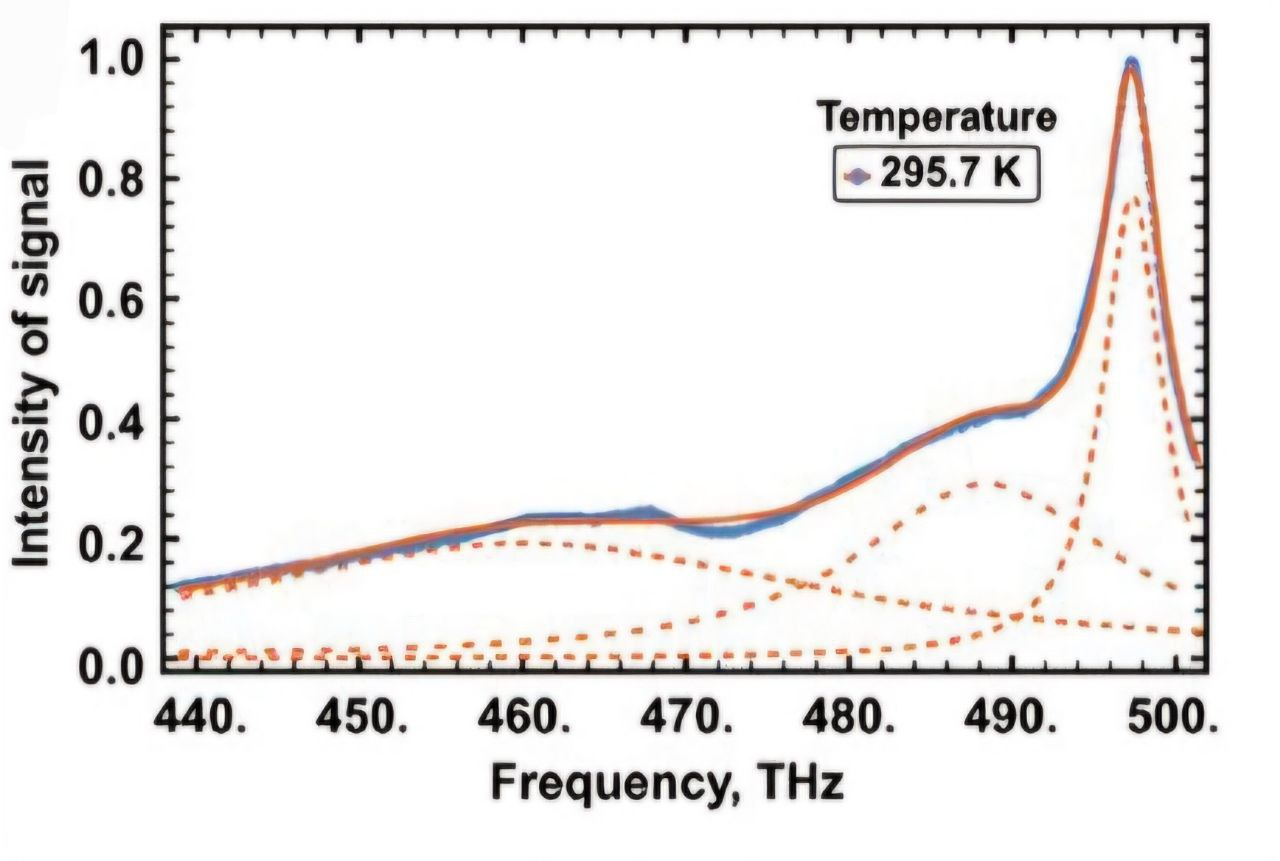
\includegraphics[width=0.7 \linewidth]{Example of fitting.jpg}
        \caption{Пример фита тремя лоренцианами. Картинка взята из статьи 
        \cite{Therm} (для GeV-центров)}
        \label{Example of fitting}
    \end{center}
\end{figure}

